
\section{threads}

\subsection{why threads?}


\begin{frame}{why threads?}
\begin{itemize}
\item concurrency: different things happening at once
    \begin{itemize}
    \item one thread per user of web server?
    \item one thread per page in web browser?
    \item one thread to play audio, one to read keyboard, \ldots?
    \item \ldots
    \end{itemize}
\item parallelism: do same thing with more resources
    \begin{itemize}
    \item multiple processors to speed-up simulation (life assignment)
    \end{itemize}
\end{itemize}
\end{frame}



\subsection{thread v. processes}

\usetikzlibrary{chains,fit,matrix}

\begin{frame}{threads versus processes}
\begin{itemize}
\item so far, was showing \myemph{each process has one thread}
\vspace{.5cm}
\item thread = part that gets run on CPU
    \begin{itemize}
    \item saved register values (including own stack pointer)
    \item save program counter
    \end{itemize}
\item rest of process
    \begin{itemize}
    \item address space (accessible memory)
    \item open files
    \item current working directory
    \item \ldots
    \end{itemize}
\end{itemize}
\end{frame}

\begin{frame}[fragile,label=singleAndMulti]{single and multithread processes}
\begin{tikzpicture}
\tikzset{
    box/.style={minimum width=1.75cm,minimum height=0.6cm,draw,thick,font=\small,fill=white},
    pcb/.style={fill=green!10},
    memory/.style={fill=yellow!10},
    tcb/.style={fill=blue!10},
}
\matrix[row sep=2.5mm,column sep=2.5mm] (sp proc) {
    \node[box,pcb] (sp files) {files}; \&
    \node[box,pcb] (sp pid) {pid}; \&
    \node[box,pcb] (sp dot) {\ldots};
    \\
    \node[box,memory] (sp code) {code}; \&
    \node[box,memory] {data}; \&
    \node[box,memory] (sp other mem) {\ldots}; \\
};
\matrix[anchor=north,row sep=2.5mm] (sp thread) at (sp proc.south) {
    \node[box,memory] (sp stack){stack}; \\
    \node[box,tcb] (sp regs) {registers}; \\
    \node[box,tcb] (sp pc) {PC}; \\
    \node[box,tcb] (sp other thread) {\ldots}; \\
};
\begin{pgfonlayer}{bg}
\node[draw,thick,fit=(sp stack) (sp other thread),inner sep=0.3mm,label={[alias=sp thread box label,font=\small]south:thread},fill=black!10] (sp thread box) {};
\end{pgfonlayer}
\node[draw,ultra thick,label={north:single-threaded process},fit=(sp proc) (sp thread) (sp thread box label)] (sp box) {};
%\node[draw=blue,ultra thick,fit=(sp files) (sp pid) (sp dot),label={north:in PCB}] {};
%\node[draw=green,ultra thick,fit=(sp code) (sp other mem) (sp stack),label={north:in memory}] {};
%\node[draw=yellow!50!black,ultra thick,fit=(sp regs) (sp tdot),label={south:in TCB or CPU}] {};
\matrix[row sep=2.5mm,column sep=2.5mm,anchor=north west] (mp proc) at ([xshift=1cm]sp proc.north east) {
    \node[box,pcb] (mp files) {files}; \&
    \node[box,pcb] (mp pid) {pid}; \&
    \node[box,pcb] (mp dot) {\ldots};
    \\
    \node[box,memory] (mp code) {code}; \&
    \node[box,memory] {data}; \&
    \node[box,memory] (mp other mem) {\ldots}; \\
};
\matrix[anchor=north,row sep=2.5mm,column sep=2.5mm] (mp threads) at (mp proc.south) {
    \node[box,memory] (mp stack 1){stack}; \& 
    \node[box,memory] (mp stack 2){stack}; \& 
    \node[box,memory] (mp stack 3){stack}; \\
    \node[box,tcb] (mp regs 1) {registers}; \&
    \node[box,tcb] (mp regs 2) {registers}; \&
    \node[box,tcb] (mp regs 3) {registers}; \\
    \node[box,tcb] (mp pc 1) {PC}; \&
    \node[box,tcb] (mp pc 2) {PC}; \&
    \node[box,tcb] (mp pc 3) {PC}; \\
    \node[box,tcb] (mp other thread 1) {\ldots}; \&
    \node[box,tcb] (mp other thread 2) {\ldots}; \&
    \node[box,tcb] (mp other thread 3) {\ldots}; \\
};
\begin{pgfonlayer}{bg}
\node[draw,thick,fit=(mp stack 1) (mp other thread 1),inner sep=0.3mm,label={[alias=mp thread box label 1,font=\small]south:thread},fill=black!10] (mp thread box 1) {};
\node[draw,thick,fit=(mp stack 2) (mp other thread 2),inner sep=0.3mm,label={[alias=mp thread box label 2,font=\small]south:thread},fill=black!10] (mp thread box 2) {};
\node[draw,thick,fit=(mp stack 3) (mp other thread 3),inner sep=0.3mm,label={[alias=mp thread box label 3,font=\small]south:thread},fill=black!10] (mp thread box 3) {};
\end{pgfonlayer}
\node[draw,ultra thick,label={north:multi-threaded process},fit=(mp proc) (mp threads) (mp thread box label 2)] (mp box) {};
\end{tikzpicture}
\end{frame}




\subsection{pthread create}

\usetikzlibrary{arrows.meta,decorations.pathmorphing,matrix}

\begin{frame}<1>[fragile,label=pthreadCreateOver]{pthread\_create}
\begin{lstlisting}[
    style=smaller,
    language=C++,
    moredelim={**[is][\btHL<2|handout:2>]{@2}{2@}},
    moredelim={**[is][\btHL<3|handout:3>]{@3}{3@}},
    moredelim={**[is][\btHL<4|handout:4>]{@4}{4@}},
    moredelim={**[is][\btHL<5|handout:5>]{@5}{5@}},
]
void *ComputePi(void *argument) { ...  }
void *PrintClassList(void *argument) { ...  }
int main() {
    pthread_t pi_thread, list_thread;
    pthread_create(&@2pi_thread2@, @4NULL4@, @3ComputePi3@, @4NULL4@);
    pthread_create(&@2list_thread2@, @4NULL4@, @3PrintClassList3@, @4NULL4@);
    ... /* more code */
}
\end{lstlisting}
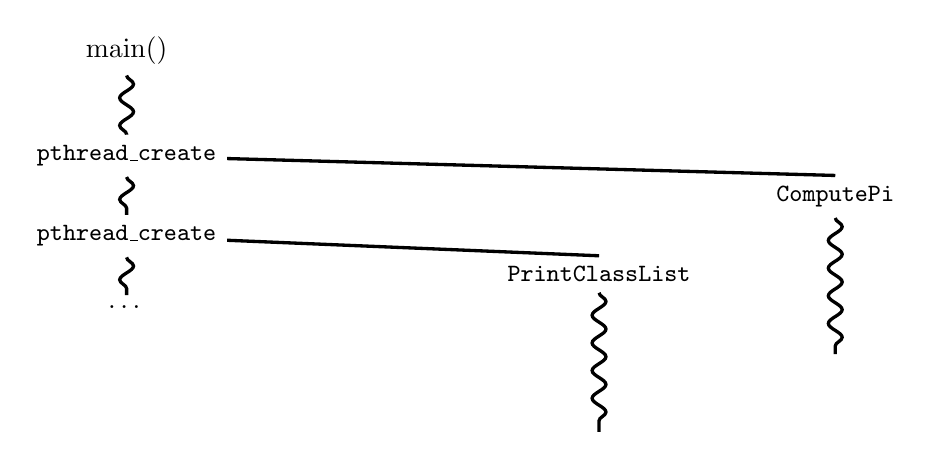
\begin{tikzpicture}
    \tikzset{
        thread/.style={very thick,draw,decorate,decoration=snake},
        split/.style={very thick,draw},
        marker/.style={thin,draw},
    }
    \draw[thread] (0, 0) node[above] {main()}-- ++(0, -.75) node[below,font=\tt\small] (create pi) {pthread\_create};
    \draw[thread] (create pi) -- ++(0, -.75) node[below,font=\tt\small] (create list) {pthread\_create};
    \draw[split] (create pi) -- ++(9, -.25) node[below,font=\tt\small] (computepi){ComputePi};
    \draw[thread] (computepi) -- ++(0, -2);
    \draw[thread] (create list) -- ++(0, -.75) node[below] {\ldots};
    \draw[split] (create list) -- ++(6, -.25) node[below,font=\tt\small] (classlist){PrintClassList};
    \draw[thread] (classlist) -- ++(0, -2);
\end{tikzpicture}
\end{frame}

\begin{frame}[fragile,label=pthreadCreateIntro]{pthread\_create}
\begin{lstlisting}[
    style=small,
    language=C++,
    moredelim={**[is][\btHL<2|handout:2>]{@2}{2@}},
    moredelim={**[is][\btHL<3|handout:3>]{@3}{3@}},
    moredelim={**[is][\btHL<4|handout:4>]{@4}{4@}},
    moredelim={**[is][\btHL<5|handout:5>]{@5}{5@}},
]
void *ComputePi(void *argument) { ...  }
void *PrintClassList(void *argument) { ...  }
int main() {
    pthread_t pi_thread, list_thread;
    pthread_create(&@2pi_thread2@, @4NULL4@, @3ComputePi3@, @4NULL4@);
    pthread_create(&@2list_thread2@, @4NULL4@, @3PrintClassList3@, @4NULL4@);
    ... /* more code */
}
\end{lstlisting}
    \begin{itemize}
    \item pthread\_create arguments:
    \item \myemph<2>{thread identifier}
    \item \myemph<3>{function to run}
        \begin{itemize}
        \item thread starts here, terminates if this function returns
        \end{itemize}
    \item \myemph<4>{thread attributes (extra settings) and function argument}
    \end{itemize}
\end{frame}




\subsection{exercise: pthread create race}
\usetikzlibrary{arrows.meta}
\begin{frame}<0>[fragile,label=pthreadCreateBrokenP]{a threading race}
\begin{lstlisting}[
    style=small,
    language=C++,
    moredelim={**[is][\btHL<1|handout:1>]{@1}{1@}},
]
#include <pthread.h>
#include <stdio.h>
void *print_message(void *ignored_argument) {
    @1printf("In the thread\n");1@ return NULL;
}
int main() {
    printf("About to start thread\n");
    pthread_t the_thread;
    pthread_create(&the_thread, NULL, print_message, NULL);
    printf("Done starting thread\n");
    return 0;
}
\end{lstlisting}
My machine: outputs \texttt{In the thread} \myemph{about 4\% of the time}. \\
What happened?
\end{frame}

\begin{frame}<0>[fragile,label=pthreadCreateRace]{a race}
\begin{itemize}
\item returning from main \myemph{exits the entire process} (all its threads)
    \begin{itemize}
    \item same as calling exit; not like other threads
    \end{itemize}
\item race: main's return 0 or print\_message's printf first?
\end{itemize}
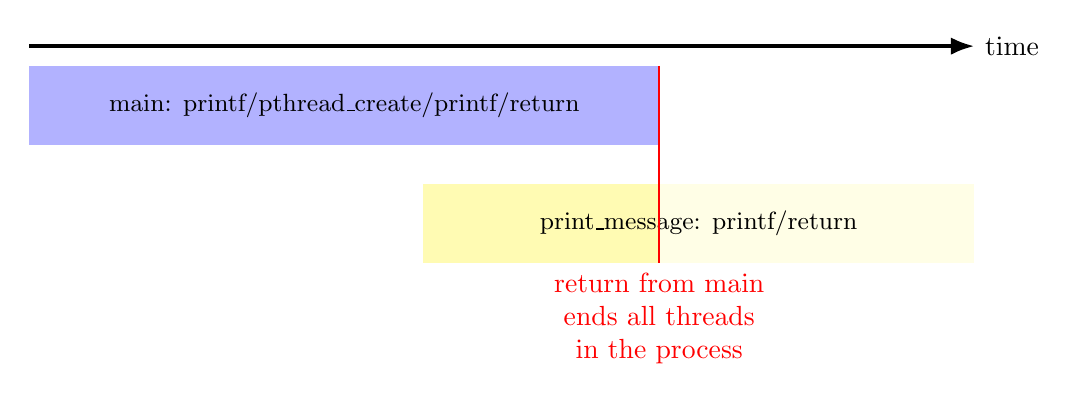
\begin{tikzpicture}
\tikzset{
    box/.style={draw,thick},
    main box/.style={fill=blue!30},
    thread box/.style={fill=yellow!30},
    my label/.style={font=\small},
    >=Latex,
}
\draw[very thick,->] (0,1.25) -- (12,1.25) node[right] {time};
\path[main box] (0, 0) rectangle (8, 1) node[midway,my label]{main: printf/pthread\_create/printf/return};
\path[thread box] (5, -.5) rectangle (8, -1.5);
\path[thread box,fill=yellow!10,dashed] (8, -.5) rectangle (12, -1.5);
\path (5, -.5) rectangle (12, -1.5) node[midway,my label]{print\_message: printf/return};
\path[draw,thick,red] (8, 1) -- (8,-1.5) node[below,align=center] {return from main \\ ends all threads \\ in the process};
\end{tikzpicture}
\end{frame}



\begin{frame}[fragile,label=pthreadCreateBrokenP]{a threading race}
\begin{lstlisting}[
    style=small,
    language=C++,
    moredelim={**[is][\btHL<1|handout:1>]{@1}{1@}},
]
#include <pthread.h>
#include <stdio.h>
void *print_message(void *ignored_argument) {
    @1printf("In the thread\n");1@ return NULL;
}
int main() {
    printf("About to start thread\n");
    pthread_t the_thread;
    pthread_create(&the_thread, NULL, print_message, NULL);
    printf("Done starting thread\n");
    return 0;
}
\end{lstlisting}
My machine: outputs \texttt{In the thread} \myemph{about 4\% of the time}. \\
What happened?
\end{frame}

\begin{frame}[fragile,label=pthreadCreateRace]{a race}
\begin{itemize}
\item returning from main \myemph{exits the entire process} (all its threads)
    \begin{itemize}
    \item same as calling exit; not like other threads
    \end{itemize}
\item race: main's return 0 or print\_message's printf first?
\end{itemize}
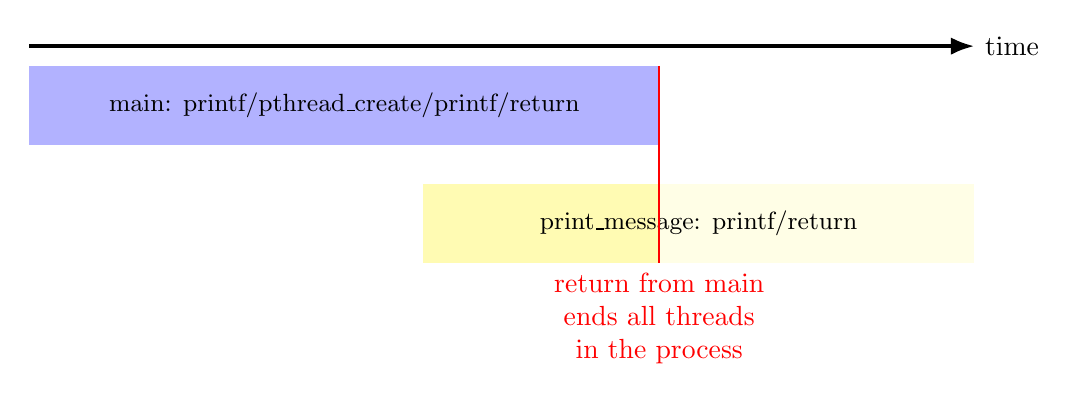
\begin{tikzpicture}
\tikzset{
    box/.style={draw,thick},
    main box/.style={fill=blue!30},
    thread box/.style={fill=yellow!30},
    my label/.style={font=\small},
    >=Latex,
}
\draw[very thick,->] (0,1.25) -- (12,1.25) node[right] {time};
\path[main box] (0, 0) rectangle (8, 1) node[midway,my label]{main: printf/pthread\_create/printf/return};
\path[thread box] (5, -.5) rectangle (8, -1.5);
\path[thread box,fill=yellow!10,dashed] (8, -.5) rectangle (12, -1.5);
\path (5, -.5) rectangle (12, -1.5) node[midway,my label]{print\_message: printf/return};
\path[draw,thick,red] (8, 1) -- (8,-1.5) node[below,align=center] {return from main \\ ends all threads \\ in the process};
\end{tikzpicture}
\end{frame}

\begin{frame}[fragile,label=fixRace1]{fixing the race (version 1)}
\begin{lstlisting}[
    style=small,
    language=C++,
    moredelim={**[is][\btHL<1|handout:1>]{@1}{1@}},
]
#include <pthread.h>
#include <stdio.h>
void *print_message(void *ignored_argument) {
    printf("In the thread\n");
    return NULL;
}
int main() {
    printf("About to start thread\n");
    pthread_t the_thread;
    pthread_create(&the_thread, NULL, print_message, NULL);
    printf("Done starting thread\n");
    @1pthread_join(the_thread, NULL);1@  /* WAIT FOR THREAD */
    return 0;
}
\end{lstlisting}
\end{frame}

\begin{frame}[fragile,label=fixRace2]{fixing the race (version 2; not recommended)}
\begin{lstlisting}[
    style=small,
    language=C++,
    moredelim={**[is][\btHL<1|handout:1>]{@1}{1@}},
]
#include <pthread.h>
#include <stdio.h>
void *print_message(void *ignored_argument) {
    printf("In the thread\n");
    return NULL;
}
int main() {
    printf("About to start thread\n");
    pthread_t the_thread;
    pthread_create(&the_thread, NULL, print_message, NULL);
    printf("Done starting thread\n");
    @1pthread_exit(NULL);1@
}
\end{lstlisting}
\end{frame}



\subsection{pthread join and exit}


\begin{frame}{pthread\_join, pthread\_exit}
\begin{itemize}
\item \texttt{pthread\_join}: wait for thread, retrieves its return value
    \begin{itemize}
    \item like \texttt{waitpid}, but for a thread
    \item return value is pointer to anything
    \end{itemize}
\item \texttt{pthread\_exit}: exit current thread, returning a value
    \begin{itemize}
    \item like \texttt{exit} or returning from main, but for a single thread
    \item same effect as returning from function passed to pthread\_create
    \end{itemize}
\end{itemize}
\end{frame}


\subsection{parallel calculations in threads}

% FIXME: slide setting up the running example

\begin{frame}[fragile,label=sumToGlobal]{sum example (only globals)}
\begin{lstlisting}[
    language=C++,basicstyle=\tt\fontsize{9}{10}\selectfont,
    moredelim={**[is][\btHL<2|handout:2>]{@2}{2@}},
    moredelim={**[is][\btHL<3|handout:3>]{@3}{3@}},
    moredelim={**[is][\btHL<4|handout:4>]{@4}{4@}},
    escapeinside=QQ,
]
int @2values[1024]2@;  int @2results[2]2@;
void *sum_front(void *ignored_argument) {
    int sum = 0;
    for (int i = @303@; i < @35123@; ++i) { sum += values[i]; }
    @4results[@303@] = sum;4@
    return NULL;
}
void *sum_back(void *ignored_argument) {
    int sum = 0;
    for (int i = @35123@; i < @310243@; ++i) { sum += values[i]; }
    @4results[@313@] = sum;4@
    return NULL;
}
int sum_all() {
    pthread_t sum_front_thread, sum_back_thread;
    /* missing: error handling */
    pthread_create(&sum_front_thread, NULL, sum_front, NULL);
    pthread_create(&sum_back_thread, NULL, sum_back, NULL);
    pthread_join(sum_front_thread, NULL); pthread_join(sum_back_thread, NULL);
    return @4results[0] + results[1]4@;
}
\end{lstlisting}
\begin{tikzpicture}[overlay,remember picture]
\tikzset{
    box/.style={draw=red,very thick,fill=white,align=left}
}
    \begin{visibleenv}<2>
    \node[box,anchor=east] at ([yshift=-1.5cm,xshift=-1cm]current page.north east) {
        values, results: global variables --- shared
    };
    \end{visibleenv}
    \begin{visibleenv}<3>
    \node[box,anchor=east] at ([yshift=-1.5cm,xshift=-1cm]current page.north east) {
        two different functions \\
        happen to be the same except for some numbers
    };
    \end{visibleenv}
    \begin{visibleenv}<4>
    \node[box,anchor=east] at ([yshift=-1.5cm,xshift=-1cm]current page.north east) {
        values returned from threads \\
        via global array instead of return value \\
        (partly to illustrate that memory is shared, \\
        partly because this pattern works when we don't join (later))
    };
    \end{visibleenv}
\end{tikzpicture}
\end{frame}



\usetikzlibrary{calc,patterns,positioning}

\newcommand{\threadSumStackDecl}{
\tikzset{
    mylabel/.style={font=\ttfamily\fontsize{9}{10}\selectfont,black!70},
    mybox/.style={draw,rectangle,minimum width=5.5cm,fill=white},
    myhigh/.style={draw,rectangle,line width=1mm, draw=blue!80!black,opacity=.3},
    hilite stack/.style={draw=red,ultra thick},
}
}
\newcommand{\threadSumFirstStack}{thread two stack}
\newcommand{\threadSumSecondStack}{thread three stack}
\newcommand{\threadSumStackObjects}{
\node[mybox,minimum height=1cm,pattern=north west lines,pattern color=black!5!white] (kernel) {Used by OS};
\begin{pgfonlayer}{bg}
\node[right=1mm of kernel.north east,mylabel] (topLabel) {0xFFFF FFFF FFFF FFFF};
\node[right=1mm of kernel.south east,mylabel] {0xFFFF 8000 0000 0000};
\end{pgfonlayer}
\node[mybox, minimum height=.5cm, below=1cm of kernel] (stack 1) {main thread stack};
\begin{pgfonlayer}{bg}
\node[right=1mm of stack 1.north east,mylabel] {0x7F\ldots{}};
\end{pgfonlayer}
\node[mybox, minimum height=.5cm, below=0.5cm of stack 1] (stack 2) {\threadSumFirstStack};
\node[mybox, minimum height=.5cm, below=0.25cm of stack 2] (stack 3) {\threadSumSecondStack};
\node[mybox, minimum height=.5cm, below=0.25cm of stack 3] (heap) {Heap / other dynamic};
\node[mybox, minimum height=.5cm, below=0mm of heap] (sdata) {Code / Data};
\begin{pgfonlayer}{bg}
\node[yshift=-1mm,right=1mm of sdata.south east,mylabel] (bottomLabel) {0x0000 0000 0040 0000};
\end{pgfonlayer}
\coordinate (memBottom) at ($(sdata.south east) + (0mm, -2mm)$);
\begin{pgfonlayer}{bg}
\draw[pattern=north west lines, pattern color=black!40!white] (kernel.north west) rectangle (memBottom);
\end{pgfonlayer}
}

\usetikzlibrary{matrix}

\begin{frame}[fragile,label=threadSumMemoryGlobals]{thread\_sum memory layout}
\begin{tikzpicture}
\threadSumStackDecl
\renewcommand{\threadSumFirstStack}{\small \texttt{sum\_front\_thread} stack}
\renewcommand{\threadSumSecondStack}{\small \texttt{sum\_back\_thread} stack}
\threadSumStackObjects
\draw[very thick,blue] ([yshift=2mm]sdata.west) rectangle ([yshift=3mm]sdata.east);
\node[anchor=west,blue!70!black] (sdata arr) at ([xshift=-1mm,yshift=4mm]sdata.east) { values, results (global) };
\begin{visibleenv}<2->
\matrix[draw,anchor=north east,tight matrix,nodes={font=\fontsize{9}{10}\selectfont,text width=2cm},
    label={[font=\fontsize{9}{10}\selectfont]north:sum\_front thread}] at
    ([xshift=8cm,yshift=4cm]sdata.east)
{
|[alias=front pc]| PC \\
|[alias=front regs]| registers \\
\ldots \\
};
\matrix[draw,anchor=north east,tight matrix,nodes={font=\fontsize{9}{10}\selectfont,text width=2cm},
    label={[font=\fontsize{9}{10}\selectfont]north:sum\_back thread}] at
    ([xshift=8cm,yshift=2cm]sdata.east)
{
|[alias=back pc]| PC \\
|[alias=back regs]| registers \\
\ldots \\
};
\draw[green!70!black,thick,<-] ([yshift=-2mm]sdata.east) -- ++(1, 0) node[right,yshift=-1mm,fill=white,font=\fontsize{10}{11}\selectfont,inner sep=0.1mm] {
        sum\_front
} -- ++(8, 0) |- ([xshift=-1cm]front pc.east);
\draw[green!70!black,thick,<-] ([yshift=0mm]sdata.east) -- ++(5, 0) node[right,fill=white,font=\fontsize{10}{11}\selectfont,inner sep=0.1mm,yshift=1mm] {
        sum\_back
} -- ++(3.25, 0) |- ([xshift=-1cm]back pc.east);
\draw[green!70!black,->] ([xshift=.5mm,yshift=1mm]front regs.west) -- ++(-3, 0) |- (stack 2.east);
\draw[green!70!black,->] ([xshift=.5mm,yshift=1mm]back regs.west) -- ++(-3, 0) |- (stack 3.east);
\end{visibleenv}
\end{tikzpicture}
\end{frame}



\subsection{passing info to threads}

\subsubsection{thread ID as argument}
% FIXME: show thread registers?

\begin{frame}[fragile,label=sumToGlobalWithId]{sum example (to global, with thread IDs)}
\begin{lstlisting}[
    language=C++,basicstyle=\tt\fontsize{9}{10}\selectfont,
    moredelim={**[is][\btHL<2|handout:2>]{@2}{2@}},
    moredelim={**[is][\btHL<3|handout:3>]{@3}{3@}},
    moredelim={**[is][\btHL<4|handout:4>]{@4}{4@}},
    escapeinside=QQ,
]
int @2values[1024]2@;
int @2results[2]2@;
void *sum_thread(void *argument) {
    int id = (int) argument;
    int sum = 0;
    for (int i = id * 512; i < (id + 1) * 512; ++i) {
        sum += values[i];
    }
    results[id] = sum;
    return NULL;
}
int sum_all() {
    /* missing: error handling */
    pthread_t thread[2];
    for (int i = 0; i < 2; ++i) {
        pthread_create(&threads[i], NULL, sum_thread, (void *) i);
    }
    for (int i = 0; i < 2; ++i)
        pthread_join(threads[i], NULL);
    return results[0] + results[1];
}
\end{lstlisting}
\begin{tikzpicture}[overlay,remember picture]
\tikzset{
    box/.style={draw=red,very thick,fill=white,align=left}
}
    \begin{visibleenv}<2>
    \node[box,anchor=east] at ([yshift=-2cm,xshift=-1cm]current page.north east) {
        values, results: global variables --- shared
    };
    \end{visibleenv}
\end{tikzpicture}
\end{frame}


\subsubsection{globals + info struct as argument}
\begin{frame}[fragile,label=sumToStack]{sum example (info struct)}
\begin{lstlisting}[
    language=C++,basicstyle=\tt\fontsize{9}{10}\selectfont,
    moredelim={**[is][\btHL<2|handout:2>]{@2}{2@}},
    moredelim={**[is][\btHL<3|handout:3>]{@3}{3@}},
    moredelim={**[is][\btHL<4|handout:4>]{@4}{4@}},
    escapeinside=QQ,
]
int @2values[1024];2@ Q\tikzmark{array}Q
struct ThreadInfo {
    int start, end, result;
};
void *sum_thread(void *argument) {
    ThreadInfo *@3my_info3@ = Q\tikzmark{info}Q (ThreadInfo *) argument;
    int sum = 0;
    for (int i = my_info->start; i < my_info->end; ++i) { sum += values[i]; }
    @4my_info->result = sum;4@
    return NULL;
}
int sum_all() {
    pthread_t thread[2]; @3ThreadInfo info[2];3@
    for (int i = 0; i < 2; ++i) {
        info[i].start = i*512; info[i].end = (i+1)*512;
        pthread_create(&threads[i], NULL, sum_thread, &info[i]);
    }
    for (int i = 0; i < 2; ++i) { pthread_join(threads[i], NULL); }
    return info[0].result + info[1].result;
}
\end{lstlisting}
\begin{tikzpicture}[overlay,remember picture]
\tikzset{
    box/.style={draw=red,very thick,fill=white,align=left}
}
    \begin{visibleenv}<2>
    \node[box,anchor=west] at (pic cs:array) {
        values: global variable --- shared
    };
    \end{visibleenv}
    \begin{visibleenv}<3>
    \node[box,anchor=north west] at (pic cs:info) {
        my\_info: pointer to sum\_all's stack \\
        only okay because sum\_all waits!
    };
    \end{visibleenv}
\end{tikzpicture}
\end{frame}

\usetikzlibrary{arrows.meta}

\begin{frame}[fragile,label=threadSumMemoryGlobalAndStacks]{thread\_sum memory layout (info struct)}
\begin{tikzpicture}
\threadSumStackDecl
\renewcommand{\threadSumFirstStack}{\small \texttt{threads[0]} stack}
\renewcommand{\threadSumSecondStack}{\small \texttt{threads[1]} stack}
\threadSumStackObjects
    \draw[very thick,blue] ([yshift=2mm]sdata.west) rectangle ([yshift=3mm]sdata.east);
    \node[anchor=west,blue!70!black] (sdata arr) at ([xshift=0cm,yshift=2.5mm]sdata.east) { values (global) };

    \node[anchor=west,blue!70!black] (info arr) at ([xshift=.5cm]stack 1.east) { info array };
    \draw[very thick,blue] ([yshift=-0mm]stack 1.west) rectangle ([yshift=-1mm]stack 1.east);

    \node[anchor=west] (my info ptr) at ([xshift=0cm]stack 2.east) { my\_info };
    \draw[-Latex] (my info ptr.east) -- ++ (1cm, 0cm) |- ([yshift=-1mm]info arr.east);
    \node[anchor=west] (my info ptr 2) at ([xshift=0cm]stack 3.east) { my\_info };
    \draw[-Latex] (my info ptr 2.east) -- ++ (1.1cm, 0cm) |- ([yshift=1mm]info arr.east);
\end{tikzpicture}
\end{frame}




\subsubsection{no globals + info struct as argument}
\begin{frame}[fragile,label=sumNoGlobals]{sum example (to main stack)}
\begin{lstlisting}[
    language=C++,basicstyle=\tt\fontsize{9}{10}\selectfont,
    moredelim={**[is][\btHL<2|handout:2>]{@2}{2@}},
    moredelim={**[is][\btHL<3|handout:3>]{@3}{3@}},
    moredelim={**[is][\btHL<4|handout:4>]{@4}{4@}},
    escapeinside=QQ,
]
struct ThreadInfo { @2int *values;2@ int start; int end; int result };
void *sum_thread(void *argument) {
    ThreadInfo *@3my_info3@ = (ThreadInfo *) argument;Q\tikzmark{info}Q
    int sum = 0;
    for (int i = my_info->start; i < my_info->end; ++i) {
        sum += my_info->values[i];
    }
    @4my_info->result = sum;4@
    return NULL;

}
int sum_all(int *values) {
    ThreadInfo info[2]; pthread_t thread[2];
    for (int i = 0; i < 2; ++i) {
        @2info[i].values = values;2@ info[i].start = i*512; info[i].end = (i+1)*512;
        pthread_create(&threads[i], NULL, sum_thread, (void *) &info[i]);
    }
    for (int i = 0; i < 2; ++i)
        pthread_join(threads[i], NULL);
    return info[0].result + info[1].result;
}
\end{lstlisting}
\end{frame}

\usetikzlibrary{arrows.meta}
\begin{frame}{program memory (to main stack)}
\begin{tikzpicture}
\threadSumStackDecl
\renewcommand{\threadSumFirstStack}{\small first thread stack}
\renewcommand{\threadSumSecondStack}{\small second thread stack}
\threadSumStackObjects

    \node[anchor=west,blue!70!black] (info arr) at ([xshift=.5cm]stack 1.east) { info array };
    \draw[very thick,blue] ([yshift=-0mm]stack 1.west) rectangle ([yshift=1mm]stack 1.east);
    \draw[-Latex] ([yshift=1.5mm]info arr.east) -- ++(2cm,0cm) node[right,yshift=0mm] { values (stack? heap?)};
    \draw[-Latex] ([yshift=-0.5mm]info arr.east) -- ++(2cm,0cm);
    
    \node[anchor=west,font=\it] (my info ptr) at ([xshift=0cm]stack 2.east) { my\_info };
    \draw[-Latex] (my info ptr.east) -- ++ (1cm, 0cm) |- ([yshift=-1mm]info arr.east);

    \node[anchor=west,font=\it] (my info ptr 2) at ([xshift=0cm]stack 3.east) { my\_info };
    \draw[-Latex] (my info ptr 2.east) -- ++ (1.25cm, 0cm) |- ([yshift=1mm]info arr.east);
\end{tikzpicture}
\end{frame}


\subsubsection{everything on the heap}
\begin{frame}[fragile,label=sumAllHeap]{sum example (on heap)}
\begin{lstlisting}[
    language=C++,basicstyle=\tt\fontsize{9}{10}\selectfont,
    moredelim={**[is][\btHL<2|handout:2>]{@2}{2@}},
    moredelim={**[is][\btHL<3|handout:3>]{@3}{3@}},
    moredelim={**[is][\btHL<4|handout:4>]{@4}{4@}},
    escapeinside=QQ,
]
struct ThreadInfo { @3pthread_t thread;3@ int *values; int start; int end; int result };
void *sum_thread(void *argument) {
    ...
}

struct ThreadInfo *start_sum_all(int *values) {
    struct ThreadInfo *info = @2calloc(2, sizeof(struct ThreadInfo);2@
    for (int i = 0; i < 2; ++i) {
        info[i].values = values; info[i].start = i*512; info[i].end = (i+1)*512;
        pthread_create(&info[i].thread, NULL, sum_thread, (void *) @2&info[i]2@);
    }
    return info;
}

int finish_sum_all(ThreadInfo *info) {
    for (int i = 0; i < 2; ++i)
        pthread_join(@3info[i].thread3@, NULL);
    int result = info[0].result + info[1].result;
    free(info);
    return result;
}
\end{lstlisting}
\end{frame}


\usetikzlibrary{arrows.meta}
\begin{frame}[fragile,label=threadSumMemoryHeap]{thread\_sum memory (heap version)}
\begin{tikzpicture}
\threadSumStackDecl
    \renewcommand{\threadSumFirstStack}{\small first thread stack}
    \renewcommand{\threadSumSecondStack}{\small second thread stack}
\threadSumStackObjects
    \node[anchor=west,blue!70!black] (info arr) at ([xshift=.5cm]heap.east) { info array };
    \draw[very thick,blue] ([yshift=-0mm]heap.west) rectangle ([yshift=1mm]heap.east);
    \draw[-Latex] ([yshift=1.5mm]info arr.east) -- ++(2cm,0cm) node[right,yshift=-1mm] { values (stack? heap?)};
    \draw[-Latex] ([yshift=-0.5mm]info arr.east) -- ++(2cm,0cm);
    \node[anchor=west,font=\it] (my info ptr 2) at ([xshift=0cm]stack 3.east) { my\_info };
    \draw[-Latex] (my info ptr 2.east) -- ++ (1.25cm, 0cm) |- ([yshift=-1mm]info arr.east);
    \node[anchor=west,font=\it] (my info ptr) at ([xshift=0cm]stack 2.east) { my\_info };
    \draw[-Latex] (my info ptr.east) -- ++ (1.5cm, 0cm) |- ([yshift=1mm]info arr.east);
\end{tikzpicture}
\end{frame}


\subsection{on thread resources, detached threads}

\subsubsection{exercise}

\usetikzlibrary{calc,decorations.pathreplacing,patterns,positioning}
\begin{frame}[fragile,label=stackLeak]{what's wrong with this?}
\begin{lstlisting}[language=C++,style=small]
/* omitted: headers */
void *create_string(void *ignored_argument) {
  char string[1024];
  ComputeString(string);
  return string;
}
int main() {
  pthread_t the_thread;
  pthread_create(&the_thread, NULL, create_string, NULL);
  char *string_ptr;
  pthread_join(the_thread, (void**) &string_ptr);
  printf("string is %s\n", string_ptr);
}
\end{lstlisting}
\end{frame}

\begin{frame}{program memory}
\begin{tikzpicture}
\tikzset{
    mylabel/.style={font=\ttfamily},
    mybox/.style={draw,rectangle,minimum width=5cm,fill=white},
    myhigh/.style={draw,rectangle,line width=1mm, draw=blue!80!black,opacity=.3},
    hilite stack/.style={draw=red,ultra thick},
}
\node[mybox,minimum height=1cm,pattern=north west lines,pattern color=black!5!white] (kernel) {Used by OS};
\begin{pgfonlayer}{bg}
\node[right=1mm of kernel.north east,mylabel] (topLabel) {0xFFFF FFFF FFFF FFFF};
\node[right=1mm of kernel.south east,mylabel] {0xFFFF 8000 0000 0000};
\end{pgfonlayer}
\node[mybox, minimum height=.5cm, below=1cm of kernel] (stack 1) {main thread stack};
\begin{pgfonlayer}{bg}
\node[right=1mm of stack 1.north east,mylabel] {0x7F\ldots{}};
\end{pgfonlayer}
\node[mybox, minimum height=.5cm, below=0.5cm of stack 1,hilite stack,alt=<2>{opacity=0.5}] (stack 2) {second thread stack};
\node[mybox, minimum height=.5cm, below=0.25cm of stack 2,hilite stack,alt=<2>{opacity=0.5}] (stack 3) {third thread stack};
\node[mybox, minimum height=.5cm, below=0.25cm of stack 3] (heap) {Heap / other dynamic};
\node[mybox, minimum height=.5cm, below=0mm of heap] (sdata) {Code / Data};
\begin{pgfonlayer}{bg}
\node[right=1mm of sdata.south east,mylabel] (bottomLabel) {0x0000 0000 0040 0000};
\end{pgfonlayer}
\coordinate (memBottom) at ($(sdata.south east) + (0mm, -2mm)$);
\begin{pgfonlayer}{bg}
\draw[pattern=north west lines, pattern color=black!40!white] (kernel.north west) rectangle (memBottom);
\end{pgfonlayer}
\draw[decorate,decoration={brace},red,ultra thick] ([xshift=.25cm]stack 2.north east) -- ([xshift=.25cm]stack 3.south east) node[midway,right,align=left](dynamicStackBox) {
    dynamically allocated stacks \\
    \texttt{char string[]} allocated here  \\
    \texttt{string\_ptr} pointed to here
};
\node[anchor=north,align=left] at ([yshift=-1cm]dynamicStackBox) {
    \ldots stacks deallocated when \\ threads exit/are joined
};
\end{tikzpicture}
\end{frame}




\subsubsection{join, detach, etc.}
\begin{frame}{thread resources}
\begin{itemize}
\item to create a thread, allocate:
\item new stack (how big???)
\item thread control block
\vspace{.5cm}
\item deallocated when \ldots
\item<2-> can deallocate stack when thread exits
\item<2-> but need to allow collecting return value
    \begin{itemize}
    \item same problem as for processes and waitpid
    \end{itemize}
\end{itemize}
\end{frame}

\begin{frame}[fragile,label=pthreadDetach]{pthread\_detach}
\begin{lstlisting}[
    style=smaller,
    language=C++,
    moredelim={**[is][\btHL<1|handout:1>]{@1}{1@}},
]
void *show_progress(void * ...) { ... }
void spawn_show_progress_thread() {
    pthread_t show_progress_thread;
    pthread_create(&show_progress_thread, NULL,
                   show_progress, NULL);

    /* instead of keeping pthread_t around to join thread later: */
    @1pthread_detach(show_progress_thread);1@
}

int main() {
    spawn_show_progress_thread();
    do_other_stuff();
    ...
}
\end{lstlisting}
\begin{tikzpicture}[overlay,remember picture]
\coordinate (place) at ([yshift=1cm]current page.south);
\node[align=left,draw=red,ultra thick,anchor=south,at={(place)}] {
    detach = don't care about return value, etc.\\
    system will deallocate when thread terminates
};
\end{tikzpicture}
\end{frame}

\begin{frame}[fragile,label=startThreadDetached]{starting threads detached}
\begin{lstlisting}[
    style=smaller,
    language=C++,
    moredelim={**[is][\btHL<1|handout:1>]{@1}{1@}},
]
void *show_progress(void * ...) { ... }
void spawn_show_progress_thread() {
    pthread_t show_progress_thread;
    pthread_attr_t attrs;
    pthread_attr_init(&attrs);
    @1pthread_attr_setdetachstate(&attrs, PTHREAD_CREATE_DETACHED);1@
    pthread_create(&show_progress_thread, attrs,
                   show_progress, NULL);
    pthread_attr_destroy(&attrs);
}
\end{lstlisting}
\end{frame}

\begin{frame}[fragile,label=setStackSize]{setting stack sizes}
\begin{lstlisting}[
    style=small,
    language=C++,
    moredelim={**[is][\btHL<1|handout:1>]{@1}{1@}},
]
void *show_progress(void * ...) { ... }
void spawn_show_progress_thread() {
    pthread_t show_progress_thread;
    pthread_attr_t attrs;
    pthread_attr_init(&attrs);
    @1pthread_attr_setstacksize(&attrs, 32 * 1024 /* bytes */);1@
    pthread_create(&show_progress_thread, attrs,
                   show_progress, NULL);
}
\end{lstlisting}
\end{frame}


\subsection{on error checking}

\begin{frame}{a note on error checking}
\begin{itemize}
\item from pthread\_create manpage:
\end{itemize}
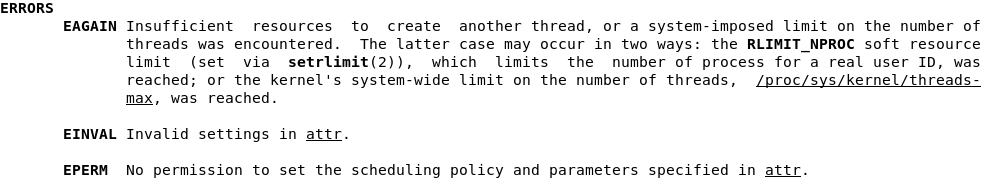
\includegraphics[width=\textwidth]{../threads/pthread-create-errors}
\begin{itemize}
\item special constants for \textit{return value}
\vspace{.5cm}
\item same pattern for many other pthreads functions
\item will often omit error checking in slides for brevity
\end{itemize}
\end{frame}

\begin{frame}[fragile,label=pthreadCreateErrorCheck]{error checking pthread\_create}
\begin{lstlisting}[language=C++,style=small]
int error = pthread_create(...);
if (error != 0) {
    /* print some error message */
}
\end{lstlisting}
\end{frame}


